\Class{Ranger}
{What you call monsters and beasts are simply other beings trying to survive in the wastelands. Some of them are just as desperate, lost, and confused as you are.}{Sudatu, elven scout}

The wastes of Athas are home to fierce and cunning creatures, from the bloodthirsty tembo to the malicious gaj. Because of that, Athasians have long learned how to adapt and survive even in the most inhospitable and savage environments.

One of the most cunning and powerful creatures of the wastes is the ranger, a skilled hunter and stalker. He knows his lands as if they were his home (as indeed they are); he knows his prey in deadly detail.

\HalfSpellcasterTable{The Ranger}{
1  & +1             & +2  & +2  & +0 & 1st favored enemy, \feat{Track}, wild empathy &&&&\\
2  & +2             & +3  & +3  & +0 & Combat style          &&&&\\
3  & +3             & +3  & +3  & +1 & \feat{Endurance}      &&&&\\
4  & +4             & +4  & +4  & +1 & Animal companion      & 0 &&&\\
5  & +5             & +4  & +4  & +1 & 2nd favored enemy     & 1 &&&\\
6  & +6/+1          & +5  & +5  & +2 & Improved combat style & 1 &&&\\
7  & +7/+2          & +5  & +5  & +2 & Woodland stride       & 2 & 0 &&\\
8  & +8/+3          & +6  & +6  & +2 & Swift tracker         & 2 & 1 &&\\
9  & +9/+4          & +6  & +6  & +3 & Evasion               & 2 & 1 &&\\
10 & +10/+5         & +7  & +7  & +3 & 3rd favored enemy     & 3 & 2 & 0 &\\
11 & +11/+6/+1      & +7  & +7  & +3 & Combat style mastery  & 3 & 2 & 1 &\\
12 & +12/+7/+2      & +8  & +8  & +4 &                       & 3 & 2 & 1 &\\
13 & +13/+8/+3      & +8  & +8  & +4 & Camouflage            & 3 & 3 & 2 & 0 \\
14 & +14/+9/+4      & +9  & +9  & +4 &                       & 3 & 3 & 2 & 1 \\
15 & +15/+10/+5     & +9  & +9  & +5 & 4th favored enemy     & 3 & 3 & 2 & 1 \\
16 & +16/+11/+6/+1  & +10 & +10 & +5 &                       & 3 & 3 & 3 & 2 \\
17 & +17/+12/+7/+2  & +10 & +10 & +5 & Hide in plain sight   & 3 & 3 & 3 & 2 \\
18 & +18/+13/+8/+3  & +11 & +11 & +6 &                       & 3 & 3 & 3 & 2 \\
19 & +19/+14/+9/+4  & +11 & +11 & +6 &                       & 3 & 3 & 3 & 3 \\
20 & +20/+15/+10/+5 & +12 & +12 & +6 & 5th favored enemy     & 3 & 3 & 3 & 3 \\
}

\subsection{Making a Ranger}
Rangers are capable in combat, although less so in open melee than the fighter, gladiator, or barbarian. His skills allow him to survive in the wilderness, to find his prey and to avoid detection. The ranger has the ability to gain special knowledge of certain types of creatures or lands. Knowledge of his enemies makes him more capable of finding and defeating those foes. Knowledge of terrain types or of specific favored lands makes it easier for him to live off the land, and makes it easier for him to take advantage of less knowledgeable foes. Rangers eventually learn to use the lesser spirits that inhabit Athas in order to produce spell-like effects. These lesser spirits inhabit small features of the land -- rocks, trees, cacti and the like.

These spirits are relatively powerless, and cannot manifest themselves. Their awareness is low, and their instincts are of the most primitive sort. The relationship between these lesser spirits and the creatures known as Spirits of the Land is unknown.

\textbf{Races:} As the race that carries the most fear and hatred of other races, and as the people with the richest land to protect, Halflings become rangers more commonly than any other race except for half-elves. Halflings are at home in their terrain (typically Forest Ridge or the Jagged Cliffs) and the ranger class teaches them the grace to move without detection, often to deadly effect. Their practice of cannibalism to emphasize their superiority over other sentient beings puts the ranger's tracking abilities to deadly use. Halfling rangers tend to take favored lands primarily, followed by favored enemy benefits. In the Forest Ridge, halfling rangers tend to pick pterrans and other neighboring races as favored enemies; rangers of the Jagged Cliffs tend to focus on bvanen, and kreen.

Elves frequently become rangers, serving as scouts and hunters for their tribes, but elves are not as naturally drawn to the wilderness as they are to magic. Half-elves are the race most compellingly drawn to the ranger class, since their isolation and natural gift with animals gives them a head start above rangers of other races. Half-Elven rangers sometimes seek to impress their Elven cousins with their desert skills, and when they are rejected, the wilderness often becomes the half-elf's only solace. A few half-elves turn to bitter hatred of the parent races that rejected them, and become merciless slave--hunters.

Although ranger skills do not come to naturally humans, their famous adaptability wins out in the end, and many humans make fine rangers. A few muls take up the ranger class while surviving in the wilderness after escaping slavery. Dwarves who become rangers find that their focus ability combines powerfully with the abilities of favored enemy and favored lands, but such characters rarely become adventurers since they tend to master wilderness skills in order to guard Dwarven communities.

Pterran rangers are common since rangers get along so well with the druidic and psionic leaders of the pterran villages. Aarakocra are similarly drawn to the ranger class to protect their villages from predators and enemies. Rangers are not unusual among the most hated humanoid races of Athas, such as gith, belgoi, and braxat. Among the various and dwindling communities of the wastes rangers are the most common character class.

\textbf{Alignment:} Rangers can be of any alignment, although they tend not to be lawful, preferring nature to civilization, silence to casual conversation, and ambush to meeting a foe boldly on the battlefield. Good rangers often serve as protectors of a village or of a wild area. In this capacity, rangers try to exterminate or drive off evil creatures that threaten the rangers' lands. Good rangers sometimes protect those who travel through the wilderness, serving sometimes as paid guides, but sometimes as unseen guardians. Neutral rangers tend to be wanderers and mercenaries, rarely tying themselves down to favored lands. The tracking and animal skills of rangers are well known in the World; virtually every trade caravan has at least one ranger scout or mekillot handler. Sometimes they stalk the land for vengeance, either for themselves or for an employer. Generally only evil rangers ply their skills in the slave trade. Other evil rangers seek to emulate nature's most fearsome predators, and take pride and pleasure in the terror that strangers take in their names.

\begin{figure*}[h!]
\centering
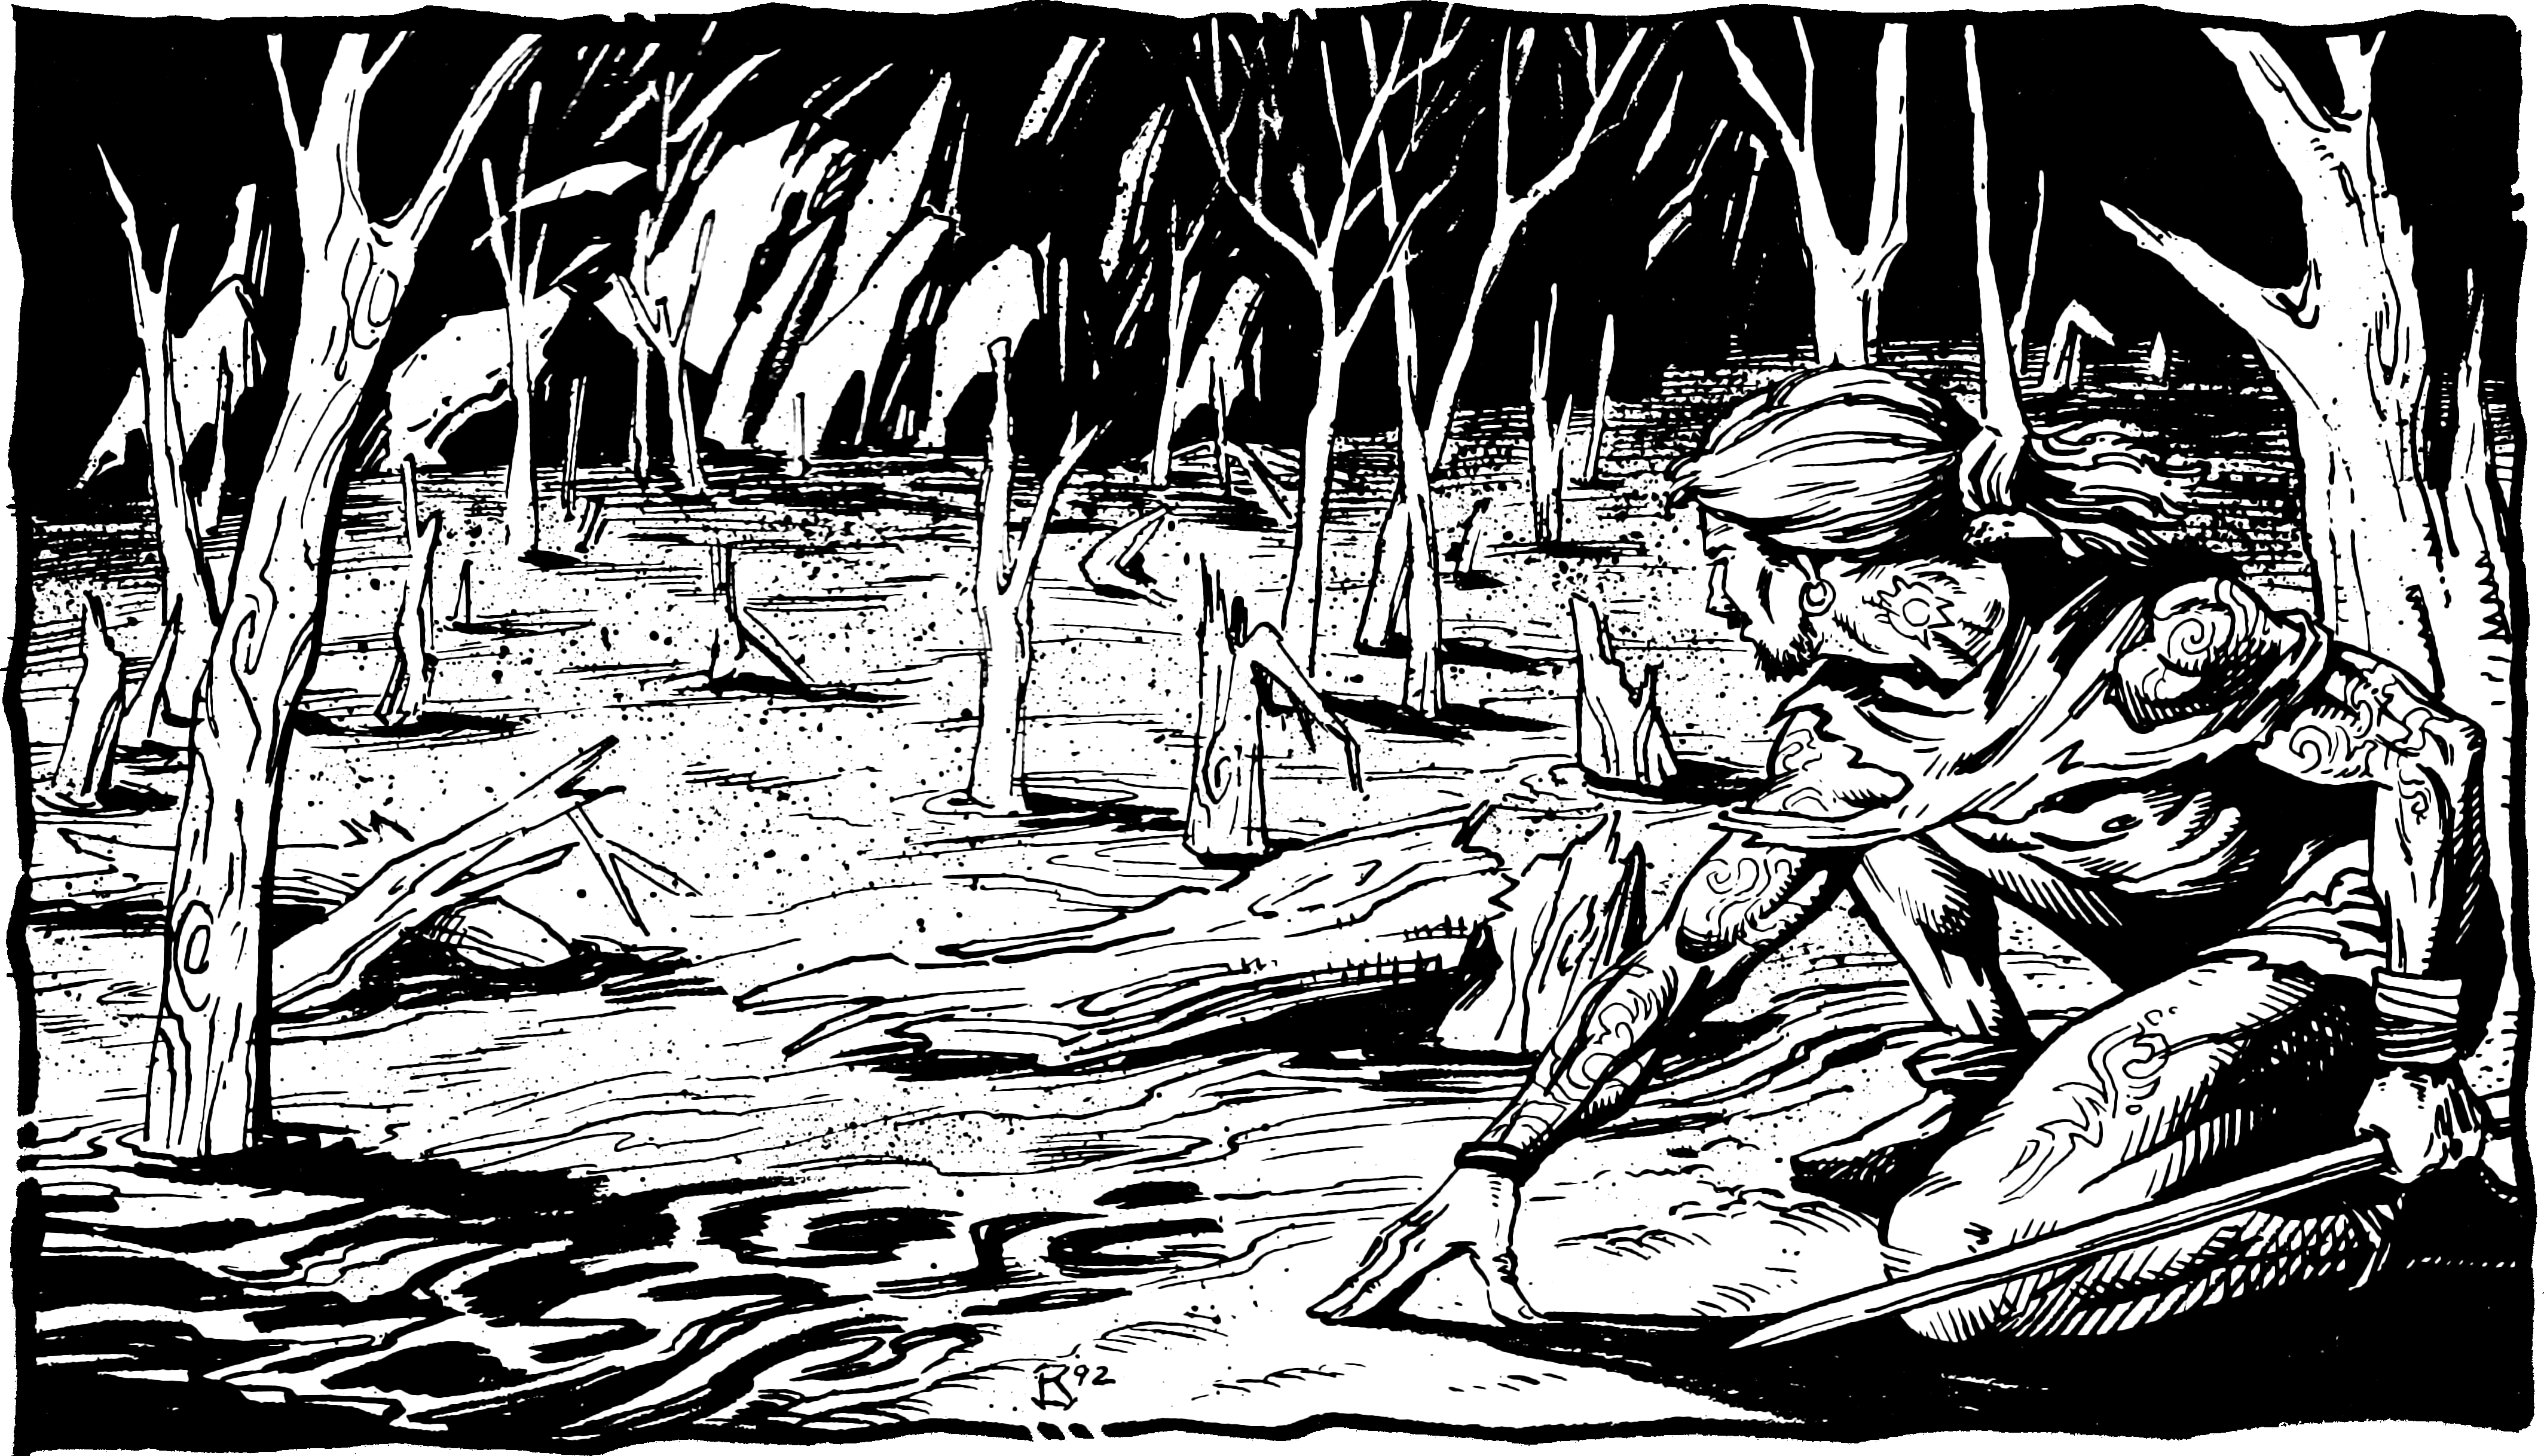
\includegraphics[width=\textwidth]{images/ranger-2.png}
\WOTC
\end{figure*}

\subsection{Game Rule Information}

\textbf{Hit Die:} d8.

\subsubsection{Class Skills}
\skill{Climb} (Str), \skill{Concentration} (Con), \skill{Craft} (Int), \skill{Handle Animal} (Cha), \skill{Heal} (Wis), \skill{Hide} (Dex), \skill{Jump} (Str), \skill{Knowledge} (dungeoneering) (Int), \skill{Knowledge} (geography) (Int), \skill{Knowledge} (nature) (Int), \skill{Listen} (Wis), \skill{Move Silently} (Dex), \skill{Profession} (Wis), \skill{Ride} (Dex), \skill{Search} (Int), \skill{Spot} (Wis), \skill{Survival} (Wis), and \skill{Use Rope} (Dex).

\textbf{Skill Points per Level:} 6 + Int modifier ($\times 4$ at 1st level).

\subsubsection{Class Features}
\textbf{Weapon and Armor Proficiency:} A ranger is proficient with all simple and martial weapons, and with light armor and shields (except tower shields).

\textbf{Favored Enemy (Ex):} At 1st level, a ranger may select a type of creature from among those given on \tabref{Athasian Favored Enemies}. The ranger gains a +2 bonus on \skill{Bluff}, \skill{Listen}, \skill{Sense Motive}, \skill{Spot}, and \skill{Survival} checks when using these skills against creatures of this type. Likewise, he gets a +2 bonus on weapon damage rolls against such creatures.

At 5th level and every five levels thereafter (10th, 15th, and 20th level), the ranger may select an additional favored enemy from those given on the table. In addition, at each such interval, the bonus against any one favored enemy (including the one just selected, if so desired) increases by 2.

If the ranger chooses humanoids or outsiders as a favored enemy, he must also choose an associated subtype, as indicated on the table. If a specific creature falls into more than one category of favored enemy, the ranger's bonuses do not stack; he simply uses whichever bonus is higher.

\textbf{Favored Terrain (Ex):} At any time when a ranger could normally select a favored enemy, he may instead choose to select a favored terrain given on \tabref{Athasian Terrains}. A ranger receives a +2 bonus on \skill{Hide}, \skill{Listen}, \skill{Move Silently}, \skill{Search}, \skill{Spot} and \skill{Survival} checks made within your favored terrain. Likewise, he gets +2 bonus on \skill{Knowledge} (geography) and \skill{Knowledge} (nature) checks about your favored terrain.

This ability uses the same graduated progression that the favored enemy ability receives.

For example, at 1st level Sudatu selects monstrous humanoids as a favored enemy, receiving a +2 bonus when combating them. At 5th level, instead of taking a new favored enemy, he selects a Rocky Badlands as his favored terrain, and chooses to increase his favored enemy bonus to +4. At 10th level, Sudatu may again choose a new Favored Enemy, and may also choose between raising his favored enemy or favored terrain bonus by +2.

\textbf{Track:} A ranger gains \feat{Track} as a bonus feat.

\Table{Athasian Favored Enemies}{X X}{
\tableheader Type (Subtype) & \tableheader Example\\
Aberration & gaj \\
Animal & lion \\
Construct & golem \\
Elemental (air) & air elemental beast \\
Elemental (earth) & crystal spider \\
Elemental (fire) & fire incarnation \\
Elemental (water) & rain paraelemental beast \\
Giant & beasthead giant \\
Humanoid (dwarf) & dwarf \\
Humanoid (elf) & elf \\
Humanoid (gith) & gith \\
Humanoid (halfling) & halfling \\
Humanoid (human) & human \\
Humanoid (jozhal) & jozhal \\
Humanoid (nikaal) & nikaal \\
Humanoid (psionic) & villichi \\
Humanoid (pterran) & pterran \\
Humanoid (reptilian) & silt runner \\
Humanoid (tarek) & tarek \\
Humanoid (tari) & tari \\
Magical beast & kirre \\
Monstrous humanoid & Thri-kreen \\
Outsider & silt half-elemental \\
Plant & hunting cactus \\
Undead & kaisharga \\
Vermin & kank \\
}

\Table{Athasian Terrains}{X X}{
\tableheader Terrain Type & \tableheader Terrain Type\\
Boulder Field & Rocky Badlands \\
Forest & Salt Flat \\
Jagged Cliffs & Sandy Wastes \\
Mountain & Sea of Silt \\
Mudflat & Stony Barrens \\
Obsidian Waste & Swamp \\
Ocean & Verdant Belt \\
}

\textbf{Wild Empathy (Ex):} A ranger can improve the attitude of an animal. This ability functions just like a \skill{Diplomacy} check to improve the attitude of a person. The ranger rolls 1d20 and adds his ranger level and his Charisma modifier to determine the wild empathy check result. The typical domestic animal has a starting attitude of indifferent, while wild animals are usually unfriendly.

To use wild empathy, the ranger and the animal must be able to study each other, which means that they must be within 9 meters of one another under normal visibility conditions. Generally, influencing an animal in this way takes 1 minute, but, as with influencing people, it might take more or less time.

The ranger can also use this ability to influence a magical beast with an Intelligence score of 1 or 2, but he takes a $-4$ penalty on the check.

\textbf{Combat Style (Ex):} At 2nd level, a ranger must select one of two combat styles to pursue: archery or two-weapon combat. This choice affects the character's class features but does not restrict his selection of feats or special abilities in any way.

If the ranger selects archery, he is treated as having the \feat{Rapid Shot} feat, even if he does not have the normal prerequisites for that feat.

If the ranger selects two-weapon combat, he is treated as having the \feat{Two-Weapon Fighting} feat, even if he does not have the normal prerequisites for that feat.

The benefits of the ranger's chosen style apply only when he wears light or no armor. He loses all benefits of his combat style when wearing medium or heavy armor.

\textbf{Endurance:} A ranger gains \feat{Endurance} as a bonus feat at 3rd level.

\textbf{Animal Companion (Ex):} At 4th level, a ranger gains an animal companion selected from the following list: lesser boneclaw, carru, dire rat, eagle, erdlu, jankx, jhakar, kes'trekel, kivit, owl, snake (Small or Medium viper). If the DM's campaign takes place wholly or partly in a silt environment, the DM may add silt spawn to the ranger's list of options. This animal is a loyal companion that accompanies the ranger on his adventures as appropriate for its kind. 

A 4th-level ranger's companion is completely typical for its kind except as noted below. As a ranger advances in level, the animal's power increases as shown on the table. If a ranger releases his companion from service, he may gain a new one by performing a ceremony requiring 24 uninterrupted hours of prayer. This ceremony can also replace an animal companion that has perished.

A ranger of 7th level or higher may select from alternative lists of animals. Should he select an animal companion from one of these alternative lists, the creature gains abilities as if the character's ranger level were lower than it actually is. Subtract the value indicated in the appropriate list header from the character's ranger level and compare the result with the ranger level entry on the table to determine the animal companion's powers. (If this adjustment would reduce the ranger's effective level to 0 or lower, he can't have that animal as a companion.)

% \textbf{Animal Companion (Ex):} At 4th level, a ranger gains an animal companion selected from the following list: badger, camel, dire rat, dog, riding dog, eagle, hawk, horse (light or heavy), owl, pony, snake (Small or Medium viper), or wolf. If the campaign takes place wholly or partly in an aquatic environment, the following creatures may be added to the ranger's list of options: manta ray, porpoise, Medium shark, and squid. This animal is a loyal companion that accompanies the ranger on his adventures as appropriate for its kind.

% This ability functions like the druid ability of the same name, except that the ranger's effective druid level is one-half his ranger level. A ranger may select from the alternative lists of animal companions just as a druid can, though again his effective druid level is half his ranger level. Like a druid, a ranger cannot select an alternative animal if the choice would reduce his effective druid level below 1st.

\textbf{Spells:} Beginning at 4th level, a ranger gains the ability to cast a small number of divine spells, which are drawn from the ranger spell list. A ranger must choose and prepare his spells in advance (see below).

To prepare or cast a spell, a ranger must have a Wisdom score equal to at least 10 + the spell level. The Difficulty Class for a saving throw against a ranger's spell is 10 + the spell level + the ranger's Wisdom modifier.

Like other spellcasters, a ranger can cast only a certain number of spells of each spell level per day. His base daily spell allotment is given on \tabref{The Ranger}. In addition, he receives bonus spells per day if he has a high Wisdom score. When \tabref{The Ranger} indicates that the ranger gets 0 spells per day of a given spell level, he gains only the bonus spells he would be entitled to based on his Wisdom score for that spell level. The ranger does not have access to any domain spells or granted powers, as a cleric does.

A ranger prepares and casts spells the way a cleric does, though he cannot lose a prepared spell to cast a cure spell in its place. A ranger may prepare and cast any spell on the ranger spell list, provided that he can cast spells of that level, but he must choose which spells to prepare during his daily meditation.

Through 3rd level, a ranger has no caster level. At 4th level and higher, his caster level is one-half his ranger level.

\textbf{Improved Combat Style (Ex):} At 6th level, a ranger's aptitude in his chosen combat style (archery or two-weapon combat) improves. If he selected archery at 2nd level, he is treated as having the \feat{Manyshot} feat, even if he does not have the normal prerequisites for that feat.

If the ranger selected two-weapon combat at 2nd level, he is treated as having the \feat{Improved Two-Weapon Fighting} feat, even if he does not have the normal prerequisites for that feat.

As before, the benefits of the ranger's chosen style apply only when he wears light or no armor. He loses all benefits of his combat style when wearing medium or heavy armor.

\textbf{Woodland Stride (Ex):} Starting at 7th level, a ranger may move through any sort of undergrowth (such as natural thorns, briars, overgrown areas, and similar terrain) at his normal speed and without taking damage or suffering any other impairment.

However, thorns, briars, and overgrown areas that are enchanted or magically manipulated to impede motion still affect him.

\textbf{Swift Tracker (Ex):} Beginning at 8th level, a ranger can move at his normal speed while following tracks without taking the normal $-5$ penalty. He takes only a $-10$ penalty (instead of the normal $-20$) when moving at up to twice normal speed while tracking.

\textbf{Evasion (Ex):} At 9th level, a ranger can avoid even magical and unusual attacks with great agility. If he makes a successful Reflex saving throw against an attack that normally deals half damage on a successful save, he instead takes no damage. Evasion can be used only if the ranger is wearing light armor or no armor. A helpless ranger does not gain the benefit of evasion.

\textbf{Combat Style Mastery (Ex):} At 11th level, a ranger's aptitude in his chosen combat style (archery or two-weapon combat) improves again. If he selected archery at 2nd level, he is treated as having the \feat{Improved Precise Shot} feat, even if he does not have the normal prerequisites for that feat.

If the ranger selected two-weapon combat at 2nd level, he is treated as having the \feat{Greater Two-Weapon Fighting} feat, even if he does not have the normal prerequisites for that feat.

As before, the benefits of the ranger's chosen style apply only when he wears light or no armor. He loses all benefits of his combat style when wearing medium or heavy armor.

\textbf{Camouflage (Ex):} A ranger of 13th level or higher can use the \skill{Hide} skill in any sort of natural terrain, even if the terrain doesn't grant cover or concealment.

\textbf{Hide in Plain Sight (Ex):} While in any sort of natural terrain, a ranger of 17th level or higher can use the \skill{Hide} skill even while being observed.


\subsubsection{The Ranger's Animal Companion}
A ranger's animal companion is different from a normal animal of its kind in many ways. A ranger's animal companion is superior to a normal animal of its kind and has special powers, as described below.

\begin{figure}[b!]
\centering
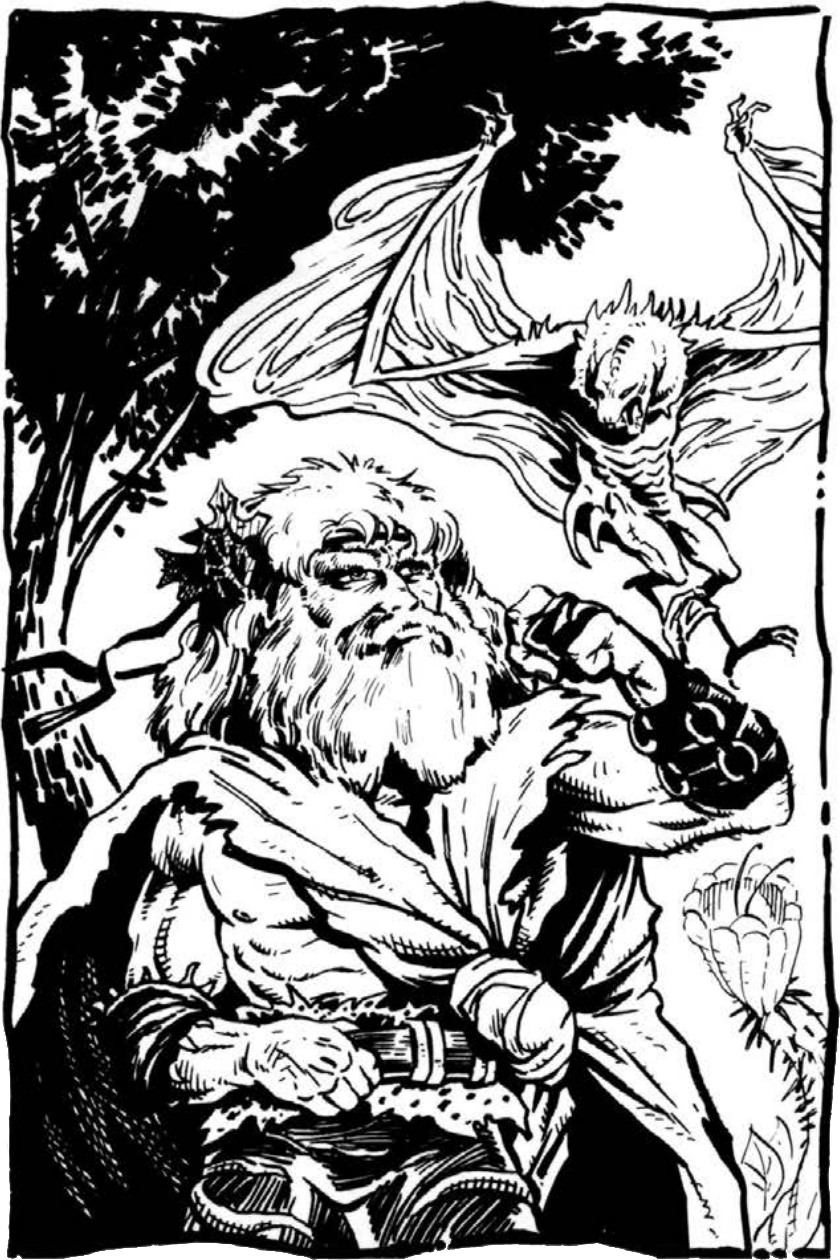
\includegraphics[width=\columnwidth]{images/druid-1.png}
\WOTC
\end{figure}

\Table{}{l Z{.5cm} Z{.8cm} Z{.8cm} Z{.7cm} X}{\tableheader Class Level & \tableheader Bonus HD & \tableheader Natural Armor Adj. &\tableheader  Str/Dex Adj. &\tableheader  Bonus Tricks &\tableheader  Special\\
4th--5th &&&& 1 & Link, share spells\\
6th--8th & +2 & +2 & +1 & 2 & Evasion\\
9th--11th & +4 & +4 & +2 & 3 & Devotion\\
12th--14th & +6 & +6 & +3 & 4 & Multiattack\\
15th--17th & +8 & +8 & +4 & 5 &\\
18th--20th & +10 & +10 & +5 & 6 & Improved evasion\\
21th--24th & +12 & +12 & +6 & 7 &}

\textbf{Animal Companion Basics:} Use the base statistics for a creature of the companion's kind, but make the following changes.

\textbf{Class Level:} The character's ranger level. The ranger's class levels stack with levels of any other classes that are entitled to an animal companion for the purpose of determining the companion's abilities and the alternative lists available to the character.

\textbf{Bonus HD:} Extra eight-sided (d8) Hit Dice, each of which gains a Constitution modifier, as normal. Remember that extra Hit Dice improve the animal companion's base attack and base save bonuses. An animal companion's base attack bonus is the same as that of a ranger of a level equal to the animal's HD. An animal companion has good Fortitude and Reflex saves (treat it as a character whose level equals the animal's HD). An animal companion gains additional skill points and feats for bonus HD as normal for advancing a monster's Hit Dice.

\textbf{Natural Armor Adj.:} The number noted here is an improvement to the animal companion's existing natural armor bonus.

\textbf{Str/Dex Adj.:} Add this value to the animal companion's Strength and Dexterity scores.

\textbf{Bonus Tricks:} The value given in this column is the total number of ``bonus'' tricks that the animal knows in addition to any that the ranger might choose to teach it (see the \skill{Handle Animal} skill). These bonus tricks don't require any training time or \skill{Handle Animal} checks, and they don't count against the normal limit of tricks known by the animal. The ranger selects these bonus tricks, and once selected, they can't be changed.

\textbf{Link (Ex):} A ranger can handle his animal companion as a free action, or push it as a move action, even if he doesn't have any ranks in the \skill{Handle Animal} skill. The ranger gains a +4 circumstance bonus on all wild empathy checks and \skill{Handle Animal} checks made regarding an animal companion.

\textbf{Share Spells (Ex):} At the ranger's option, he may have any spell (but not any spell-like ability) he casts upon himself also affect his animal companion. The animal companion must be within 1.5 meter of him at the time of casting to receive the benefit. If the spell or effect has a duration other than instantaneous, it stops affecting the animal companion if the companion moves farther than 1.5 meter away and will not affect the animal again, even if it returns to the ranger before the duration expires.

Additionally, the ranger may cast a spell with a target of ``You'' on his animal companion (as a touch range spell) instead of on himself. A ranger and his animal companion can share spells even if the spells normally do not affect creatures of the companion's type (animal).

\textbf{Evasion (Ex):} If an animal companion is subjected to an attack that normally allows a Reflex saving throw for half damage, it takes no damage if it makes a successful saving throw.

\textbf{Devotion (Ex):} An animal companion gains a +4 morale bonus on Will saves against enchantment spells and effects.

\textbf{Multiattack:} An animal companion gains \feat{Multiattack} as a bonus feat if it has three or more natural attacks and does not already have that feat. If it does not have the requisite three or more natural attacks, the animal companion instead gains a second attack with its primary natural weapon, albeit at a $-5$ penalty.

\textbf{Improved Evasion (Ex):} When subjected to an attack that normally allows a Reflex saving throw for half damage, an animal companion takes no damage if it makes a successful saving throw and only half damage if the saving throw fails.

\subsubsection{Alternative Animal Companions}
A ranger of sufficiently high level can select his animal companion from one of the following lists, applying the indicated adjustment to the ranger's level (in parentheses) for purposes of determining the companion's characteristics and special abilities.

Some animals are only available in certain environments. The animals available only in an aquatic environment, such as the Last Sea, are marked with $\dagger$. The animals available only in a silt environment, such as the Sea of Silt, are marked with $\diamond$.

\Table{}{X X}{
\multicolumn{2}{c}{\tableheader\footnotesize 7th Level or Higher (Level $-6$)}\\
Carru, bull (6HD) & Leopard \\
Cheetah & Lizard, giant \\
Crodlu & Lizard, monitor\\
Crodlu, heavy & Rasclinn\\
Dire bat & Athasian shark$^\dagger$\\
Erdland & Snake, constrictor\\
Jhakar, Medium (6HD) & Snake, viper (Large)\\
Kluzd & }
\Table{}{X X}{
\multicolumn{2}{c}{\tableheader\footnotesize 10th Level or Higher (Level $-9$)}\\
Crodlu, heavy warmount & Puddingfish$^\dagger$ \\
Inix & Lion\\
Kalin & Lizard, subterranean\\
Kluzd (7HD) & Snake, viper (Huge)\\
Lirr & Takis\\
Pterrax & Tiger}
\Table{}{X X}{
\multicolumn{2}{c}{\tableheader\footnotesize 13th Level or Higher (Level $-12$)}\\
Cha'thrang & Lizard, minotaur\\
Dire lion & Athasian shark (Huge)$^\dagger$ \\
Hatori & Snake, giant constrictor}
\Table{}{X X}{
\multicolumn{2}{c}{\tableheader\footnotesize 16th Level or Higher (Level $-15$)}\\
Lirr, large (11HD) & Athasian sloth\\
Ruktoi$^\diamond$ & }
\Table{}{X X}{
\multicolumn{2}{c}{\tableheader\footnotesize 19th Level or Higher (Level $-18$)}\\
Dire Athasian shark$^\dagger$ & Silt Horror, white$^\diamond$\\
Dire tiger & Slimahacc\\
Hatori, gargantuan (17HD) & \\
}

\subsection{Playing a Ranger}

As a ranger, you nurture a close, almost mystical connection to the deadly terrain of Athas. To you, the burnt landscape is not a friend, but a well-respected adversary. Danger is always present, yet you understand it and even find a certain succor in living alongside it.

\subsubsection{Religion}

Many rangers pay homage to the elements, but a greater number honor the moons and the stars that guide them in the night---even though these celestial bodies do not have priests. In several city-states, particularly Gulg,
Kurn, and Eldaarich, many rangers owe fealty to the sorcerer-kings---virtually the entire noble caste of Gulg is comprised of rangers called judaga. Some rangers pay patronage to the Spirits of the Land, although these spirits do not bestow spells on rangers except those that multi-class as druid.

\subsubsection{Other Classes}

Rangers are slow to make friends with anyone, but have a particular affinity to druids, and to a lesser extent, barbarians and psions. Rangers tend not to lean on others for support and friendship, and often find it difficult to tolerate others who are quite different from themselves, such as talkative traders or controlling templars. Good rangers might simply try to avoid sharing a watch with a character that annoys them; neutral rangers tend to abandon annoying companions or just let them die; while evil rangers act friendly to the annoying companion and then slit their throat in their sleep.

Good rangers tend to hate defilers, although many rangers are ignorant of the distinction between preserving and defiling and hate wizards of all stripes. Strangely, many rangers have little objection to taking a companion who is of a favored enemy race, so long as that they are convinced that the companion is trustworthy and loyal.

\subsubsection{Combat}

Although you are a formidable warrior, you usually prefer not to stand against the sheer might of Athas' fighter, barbarians and gladiators. Your greatest ally is the environment itself. While in you favored terrain, you have a clear advantage over your adversaries. Try choosing favored enemies that are more common in your favored terrain.

As you advance, you are well served to invest in spells that have an effect other than dealing damage. If you can't drop a foe in one or two attacks, you can use entangle, snare, sting of the gold scorpion, or the like to make your opponents less dangerous in a prolonged fight.

\subsubsection{Advancement}

Perhaps the most dangerous place in Athas is inside a city-state: an environment rife with political intrigue, diseases, and assassination. To escape these noxious environs, you sought refuge in the wild where even the foulest elements of a society fear to tread. By gaining an intimate knowledge of this hazardous realm, you buy some breathing room and security from the urban madness.

As your ranger abilities increase, you find the Athasian wilderness a more and more inviting place (if a place with such constant peril can be called inviting). You can use your skills to establish safe havens for yourself or to gain employment opportunities---perhaps guiding a group of recently caught slaves through the Tyr valley or some noble into distant dangerous, location. You can also find that continuing to advance as a ranger or barbarian augments your already impressive abilities in the Athasian lands.

Continue to focus on skills such as \skill{Hide}, \skill{Move Silently}, and \skill{Survival}. Spend discovered treasure on poison, magic weapons, and protective magic. The \feat{Mobility} feat is good to consider, as is \feat{Nature's Child} or \feat{Wastelander}.

\subsection{Starting Packages}
\subsubsection{The Archer}
Elf Ranger

\textbf{Ability Scores:} Str 14, Dex 17, Con 10, Int 10, Wis 13, Cha 8.

\textbf{Skills:} \skill{Hide}, \skill{Listen}, \skill{Move Silently}, \skill{Spot}, \skill{Survival}.

\textbf{Languages:} Common, Elven.

\textbf{Feat:} \feat{Point Blank Shot}, \feat{Track}.

\textbf{Weapons:} Macahuitl (1d8/19--20)

Longbow with 20 arrows (1d8/$\times$3, 30 m).

\textbf{Armor:} Studded leather (+3 AC).

\textbf{Other Gear:} Standard adventurer's kit, 19 cp.

\subsubsection{The Scout}
Halfling Ranger

\textbf{Ability Scores:} Str 11, Dex 17, Con 12, Int 10, Wis 14, Cha 8.

\textbf{Skills:} \skill{Hide}, \skill{Knowledge} (nature), \skill{Listen}, \skill{Move Silently}, \skill{Spot}, \skill{Survival}.

\textbf{Languages:} Halfling.

\textbf{Feat:} \feat{Stealthy}, \feat{Track}.

\textbf{Weapons:} Macahuitl (1d6/19--20)

Small macahuitl (1d3/19--20)

Five javelins (1d4, 9 m).

\textbf{Armor:} Studded leather (+3 AC).

\textbf{Other Gear:} Standard adventurer's kit, 65 cp.

\subsubsection{The Wastelander}
Thri-kreen Ranger

\textbf{Ability Scores:} Str 14, Dex 19, Con 14, Int 8, Wis 15, Cha 4.

\textbf{Skills:} \skill{Hide}, \skill{Knowledge} (nature), \skill{Listen}, \skill{Move Silently}, \skill{Spot}, \skill{Survival}.

\textbf{Languages:} Kreen.

\textbf{Feat:} \feat{Track}, \feat{Wastelander}.

\textbf{Weapons:} Gythka (1d8/1d8)

Three chatkchas (1d6, 6 m).

\textbf{Armor:} Studded leather (+3 AC).

\textbf{Other Gear:} Standard adventurer's kit, 5 cp.

\subsection{Rangers on Athas}
\Quote{Trust me. He might not talk a lot and smell funnier than the rest of your men, but there is no other one I would bring along with me around the Great Ivory Plains.}{Waltian Inika, Gulg dune trader}

The Athasian wilderness is harsh and unforgiving, calling for skilled and capable men to master its ways---the ranger answers that challenge, living a rugged life through clever mastery of his surroundings. The ranger has a potent combination of stealth, woodcraft, magic, and fighting skill, making him the master of the wilderness.

\subsubsection{Daily Life}

A ranger adventures to learn about Athas, to protect nature, and to prove his superior hunting skills. Rangers spend their days in contemplation of nature, and tending their animal companions.

The Athasian ranger is a wanderer who hunts down a defiler to avenge himself for having his village destroyed, or a mercenary hunter for both monsters and humanoid creatures, or even a loner who simply prefers the company of animals.

\subsubsection{Notables}

Tales of halfling snipers are among the common Athasian legends. Any traveler to the Forest Ridge should rightfully fear the cannibals that move without a sound and strike without being seen. Thri-kreen are fabled for their rangers, as they are fast-moving relentless natural hunters, and their unarmed combat abilities become even more deadly when applied to subduing a quarry.

\subsubsection{Organizations}

There is no organized ranger organization; you are most likely to be a loner---or at best the leader of a group of raiders or renegades---than you are to gather with other rangers.

Often merchant houses are eager to employ you as a caravan guide through the most dangerous trade routes, or a city-state's templarate might hire you to provide a safe path to a templar patrol.

\subsubsection{NPC Reactions}

Within a city-state or large settlement, you find that you are either ignored or regarded with some small amount of curiosity. It is only after a city-dweller find himself outside the boundaries of his city-state that he truly appreciates you. Indeed, he holds you in the highest of regards, knowing that you are all that stands between him and a horrible death in the wastes.

\subsubsection{Ranger Lore}

Characters with ranks in \skill{Knowledge} (nature) can research rangers to learn more about them. When a character makes a skill check, read or paraphrase the following, including the information from lower DCs.

\textbf{DC 10:} Only those assisted by a ranger can hope to survive in the Athasian wilderness for long.

\textbf{DC 15:} Rangers move with ease through the harsh terrains that others find dangerous or impassable. They make of this aptitude to specialize in battling specific creatures of the wild.

\textbf{DC 20:} As a ranger advances in knowledge and skill, he grows more and more connected to the land, and eventually manages to draw spells from it.
